\chapter[Literature Review]{Literature Review}
\vspace{12pt}

To better understand the current progress in mobile ad-hoc network technology, let's look into the current findings and ongoing research in the fields of networking. There are some interesting researches done in these fields which can be used to find an answer to the above research problem.

\vspace{12pt}

\subsection{COMONet: Community Mobile Network}

\vspace{12pt}

One of the focuses of research being conducted in the field of ad-hoc networks is in making networking more flexible, both on the physical network side and the application side, as with most applications nowadays being developed with infrastructure networks and always-on connectivity in mind.
\vspace{12pt}

When smartphones were introduced, there were no open software devices like Android available to the public. Smartphone industry was dominated by closed echo system devices. back then Symbian Ltd(2019, Aug)What is Symbian OS https://www.symbianos.org/ \cite{SymbianOS} was the go-to OS choice for mobile devices. originated from EPOC32, an operating system created by Psion in the 1990s. In June 1998, Psion Software became Symbian Ltd. It was a major joint venture between Psion and phone manufacturers  Ericsson, Motorola, and Nokia. So due to the close nature in software and hardware of those devices, modifying them to create an ad-hoc network was not an easy task back then.

\vspace{12pt}
Project COMONet(Wijesekera and Keppitiyagama 2007)\cite{comonet} was undertaken in this kind of environment back then. COMONet was a  Community based  Mobile Network which utilizes Wi-Fi and Bluetooth interfaces to build an Ad-Hoc network among mobile phone users to bypass GSM base stations whenever possible. It provided the functionality to make voice calls without the help of a carrier network.

\vspace{12pt}
\pagebreak
To use this functionality caller and the callee does not have to be within the Wi-Fi or Bluetooth range of each other to make a call since the COMONet(Wijesekera and Keppitiyagama 2007)\cite{comonet} is capable of routing calls through the other mobile nodes that are participating in the network. It can switch in between mesh connection and the cellular connection on the fly without breaking the connection.

\vspace{12pt}

Let us dig deeper into the implementation of the COMONet. What the researcher has done hear was to implement a mobile ad-hoc mesh network using the readily available network interfaces of the mobile devices. 
COMONet uses different networking stacks to implement the vice call functionality as shown in Figure \ref{fig: Wireless View of COMONet} below.
\vspace{12pt}

\begin{figure}[H]
    \centering
   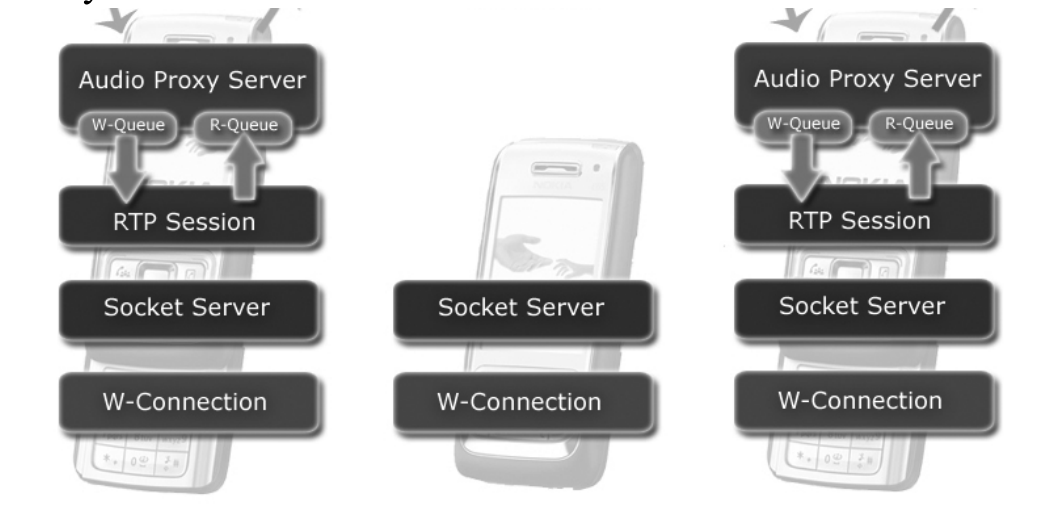
\includegraphics[scale=0.6]{comonet_wireless_view.png}
    \caption{Wireless View of COMONet(Source COMONet\cite{comonet})}
    \label{fig:Wireless View of COMONet}
\end{figure}

\vspace{12pt}

Most of the functionalities in the above stack are not readily available to the application developer. So to get access to the networking interfaces to ring 0 privileges is a must.  What the researcher had done is to use a hack to get into kernel mode and passing that data out to the application layer to use with his device. Believe me, this is no easy task to do. One way to do this is to read the machine code of the OS and modifying the relevant bits so that it gives the elevated (ring 0) privileges to the Comment app. To my knowledge, this is not a good design because if the COMONet application crashes, then the whole os crashes. But at that time this was not feasible to in the proper manner due to the closed nature of the Symbian ecosystem.


\vspace{12pt}
\pagebreak
\subsection{The SPAN project: SmartPhone Ad-Hoc Networks}

\vspace{12pt}

The SPAN project(Thomas, et al.2012)\cite{defcon_paper} utilizes MANET (Mobile Ad-Hoc Network) technology to provide a resilient backup framework for communication between two devices when all other infrastructure is unavailable or unreliable. The MANET based solution is a headless, infrastructure-less network that allows common smartphones to link together in a dynamic way to create a mobile ad-hoc network.

\vspace{12pt}

They have injected the framework into the existing Android network stack between OSI layers 2 and 3 as shown in Figure \ref{fig:span}. Privileges needed to create the ad-hoc network is gained by accessing the wireless chip drivers directly to set the parameters of the wireless interface. They have configured the wireless chip to work in ad-hoc mode by using the iwconfig Linux command-line utility.The Debian Project(2019,Aug) Official WIKI page https://wiki.debian.org/iwconfig \cite{iwconfig}

\vspace{12pt}

They have customized the device network drivers in this implementation. By doing so they have limited the generalizability of the technology in different devices. Plus side of implementing the network in this manner is that it can change the routing protocol in a dynamic passion. To my knowledge, most of the ad-hoc implementations cannot achieve this feature.


\vspace{12pt}



\begin{figure}[H]
    \centering
   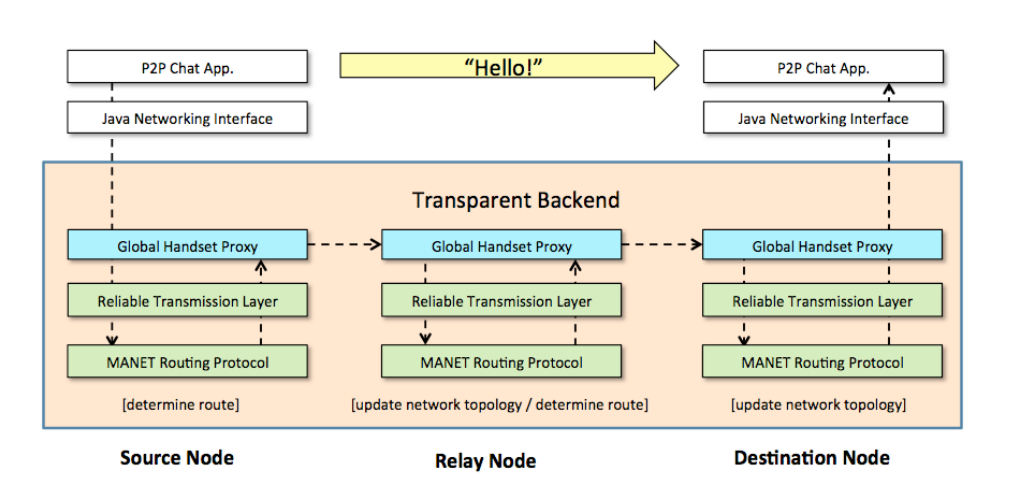
\includegraphics[scale=0.8]{span.png}
    \caption{Cross-sectional view of the network(Source SPAN Project\cite{defcon_paper})}
    \label{fig:span}
\end{figure}
\vspace{12pt}
\pagebreak

\subsection{Better approach to mobile ad-hoc networking}

\vspace{12pt}
BATMAN project: A better approach to mobile ad-hoc networking
\cite{BATMAN} by Open Mesh organization is a routing protocol for multi-hop ad-hoc mesh networks. People at Open-Mesh have implemented this framework to support local routing on top of the ad-hoc enabled kernel. Open Mesh (2019,Aug) B.A.T.M.A.N. project https://www.open-mesh.org/projects/batman-adv/

\vspace{12pt}


This system works on top of the kernel to support ad-hoc routing by modifying the messages passed inside the network environment. Initially, they flood the network with announcement messages. So every node knows who their neighbours are. Due to this if there was a missing node we only need to change the routing data of the local nodes. Besides routing, the framework provides other functionalities such as benchmarking the network and node visualization.

\vspace{12pt}

As they have to implement the platforms on top of an ad-hoc enabled kernel this cannot use with a normal stock Android device. To use this framework we need a custom  Android OS like Lineage OS. Lineage OS Team(2019,March)\cite{lineageOS}. They haven't automated the process of creating the network yet. So this is not a user-friendly solution as well. The efficiency of their protocol has been discussed in their documentation. To my knowledge, this is pretty efficient at routing data. We cannot use this in our research due to the limited number of the devices that they support. 




\vspace{12pt}



\subsection{Mobile Ad-hoc Networks over Wi-Fi Direct}

%{Development of Mobile Ad-hoc Networks over Wi-Fi Direct with Off-the-Shelf Android Phones (Liu, et al.2016)\cite{GO}}

\vspace{12pt}
In this paper, researchers try to introduce a novel method to achieve multi-hop communication among open-source, non-rooted Android devices using Wi-Fi Direct Technology. This solution tries to preserve the ad-hoc property of the network while utilizing minimum privileges. (Liu, et al.2016)\cite{GO}

\vspace{12pt}


Let us analyze this method. They have chosen the  WIFI  interface for their communication. Bluetooth interface has been discarded due to its low bandwidth rates. The protocol he had chosen here is the WIFI-Direct. It allows them to create groups inside the network. Initially, all the nodes become group owners. When it is time to transfer the message some becomes clients. After the message has been transferred node revert back to its initial state.

\vspace{12pt}

This method preserves the ad-hoc nature of the network. But because in each transfer of data it needs to make and break the structure of the network transfer rates becomes low. Due to this, it is pretty hard to keep a continuous stream of data using this network.

\vspace{12pt}



\subsection{Enabling multi-hop ad-hoc through  WIFI  direct multi-group networking}{Enabling multi-hop ad hoc networks through  WIFI  direct multi-group networking (Heinzelman et al.)\cite{wifi-direct_and_hotspot} }

\vspace{12pt}

In this paper, Heinzelman et al.\cite{wifi-direct_and_hotspot} and have proposed and analyzed different practical solutions for supporting the communications between multiple WIFI  Direct groups using Android OS devices. They have analyzed the WIFI Direct standard and the limitations of the current implementation of the Android WIFI  Direct framework and presented some possible solutions to interconnect different groups to create multi-hop ad hoc networks.

\vspace{12pt}

Let us consider their proposed method to create multi-hop ad hoc networks. In this method near devices are connected using WIFI-Direct architecture (Group owner and Client). Intergroup communication is achieved using this WIFI-Direct protocol. They have used the hotspot functionality of the Android to achieve intergroup communication. To do this they need to allocate a node to provide hotspot functionality to other groups. To enable inter-group communication they have modified the routing table of relevant devices. To do this the root access to the device is needed.
\vspace{12pt}


In this implementation, they have done no modifications to the operating system. They have modified the routing tables of certain devices to achieve intergroup communication. This needs root access for modification of the routing table. This limits the usability of this system in personal devices as rooting voids the warranty of most of the Android devices.

\vspace{12pt}



\subsection{Infrastructure-less Communication Platform for Android}


%{infrastructure-less Communication Platform for Off-The-Shelf Android Smartphones : (Takuo et al.)\cite{wif_direct_with_relay_nodes} }

\vspace{12pt}

In this research, they are trying to implement an ad-hoc network without modifying the OS or rooting the Android device.  They have introduced new topology for the network and relevant routing protocols to go along with that. They have used WIFI-Direct and WIFI interfaces to implement the network.


\vspace{12pt}

The researchers(Takuo et al.)\cite{wif_direct_with_relay_nodes} have made some interesting trade-off between architecture, performance and the required privilege levels when implementing this network. They have used a tree architecture Figure \ref{fig:topology_construction} rather than a graph architecture when designing the network. They proposed a relay node to do the inter-cluster communication. This relay node uses the WIFI  connection to transfer the data from one device to another. Other message transfers use the WIFI -direct protocol.
\vspace{12pt}

\begin{figure}[H]
    \centering
    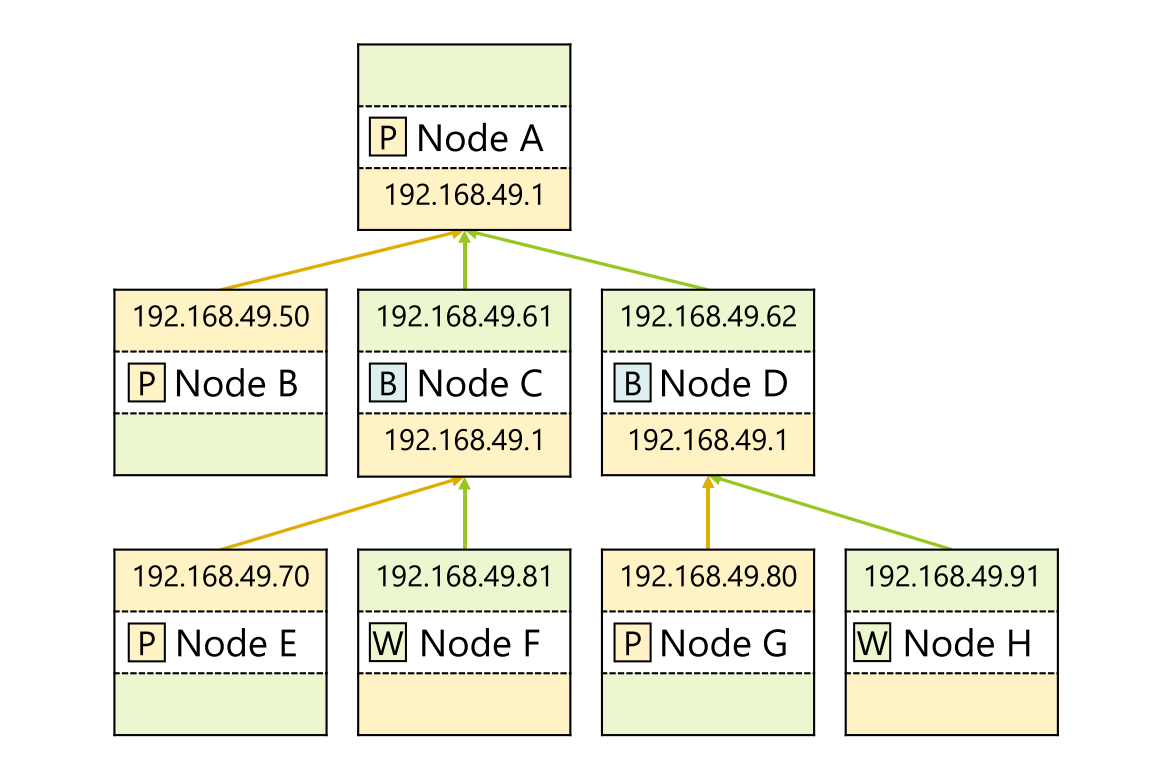
\includegraphics[scale=0.65]{network_topology_with_relay_node.png}
    \caption{Example of topology construction}
    \label{fig:topology_construction}
\end{figure}

\vspace{12pt}
Because of the topology, they proposed the network will have a low latency connection and high bandwidth. But due to the non-distributed nature of the relay node, it takes some time to recover from a node failure. Implementing this network does not need any  OS-level modifications or root privileges. Allocation of a relay node is not a good approach because that device cannot be a user in this network.

\vspace{12pt}
\subsection{Integrated Cellular and Ad Hoc Relaying Systems}

\vspace{12pt}
In this paper, they have proposed the idea of using ad-hoc and cellular connection side by side to improve the quality of the connection. In this architecture, the two networks do not talk to each other. But in my research cellular connection is used to make the ad-hoc network. And in the above research, they are concerned only on the theoretical aspect of the network. (Tonguz at el. 2001)\cite{iCAR}

\vspace{12pt}

\subsection{WiFi Direct and LTE D2D in Action}

\vspace{12pt}
In this paper, they have proposed the method of using the WIFI  direct and cellular connection side by side to improve the bandwidth of the connection. But here they are more interested in the implementation aspects of the network rather than the theoretical aspects. In this paper, they have analyzed the nature of the connection using different criteria as well. (Arash and Vincenzo 2013)\cite{wifi_direct_lte}

\vspace{12pt}

\subsection{A Unified Cellular and Ad-Hoc Network Architecture}

%{UCAN: A Unified Cellular and Ad-Hoc Network Architecture (Haiyun, Ramachandran, Prasun and Erran,2003)\cite{UCAN}}

\vspace{12pt}
In this research (Erran at el.2003)\cite{UCAN} have introduced an implementation of a hybrid ad-hoc cellular network. It answers the question can these two networks be synergistically combined to leverage the advantages of each other. 

\vspace{12pt}



\subsection{Routing Protocols in an Ad-hoc network}

%{Routing protocols in an ad-hoc network (Casetti, et al.2015)\cite{content_centric}}

\vspace{12pt}
In the paper by (Casetti, et al.2015)\cite{content_centric}, they have proposed a content-centric routing algorithm that can be used in a mobile ad-hoc network. In this method, the content delivery leverages the forwarding scheme through a content-centric approach.

\vspace{12pt}
In the paper by (Philippe, Muhlethaler, Clausen and Laouiti)\cite{olsr}, they have analyzed the use of OLSR(Optimized Link State Routing) protocol in an ad-hoc routing environment. This is a proactive routing protocol for mobile ad hoc networks.OLSR protocol is an optimization of a pure link-state protocol for mobile ad hoc networks. This technique significantly reduces the number of retransmissions in a flooding or broadcast procedure.

\vspace{12pt}

The paper A Study of Ad-Hoc Networks by (Alshaer and El-Rabaie)\cite{adhoc_survay} does some higher-level analysis of the routing protocol that can be used with a mobile ad-hoc network. In this paper, researchers analyze how different aspects of the network affect these protocols.

\vspace{12pt}

\subsection{Secure Key Establishment for Device Communications }

%{Secure Key Establishment for Device-to-Device Communications (yin)\cite{Security}}

\vspace{12pt}
In this paper, researchers(yin at el.)\cite{Security} investigate the security requirements and challenges for a device to device communications and present a secure and efficient key agreement protocol, which enables two mobile devices to establish a shared secret key for D2D communications without prior knowledge

\vspace{12pt}





\section{Summary }

\vspace{12pt}
Several efforts are in development to address many of the requirements to achieve decentralised mobile ad-hoc networking. Some researchers are based on implementation aspects of the network and others are focused on the theoretical aspects of the network.
\vspace{12pt}
Initially, we discussed different ways we can make an ad-hoc network. This can from complete OS modification, routing table modification to application-level modification with no additional privileges(no root). Most recent implementations rely on WIFI  direct protocol to implement ad-hoc networking. When designing the architecture we need to concern the modification that needs to be done on an Android system because of this affect the reach of our research.


\vspace{12pt}

In the later part, we discuss different kinds of cellular ad-hoc hybrid network and their performance in a theoretical and practical manner. The current implementations of ad-hoc network targets on Android devices relying on new and/or proprietary standards, ignoring the existing standards used across many existing implementations. This limits their use unless they gain mass-market adoption


\vspace{12pt}

\pagebreak












